%\chapter{Supplemental Figures} \label{sec:suppfigs}
\chapter{Restoring force on Bead Handles}

\begin{figure}
\centering
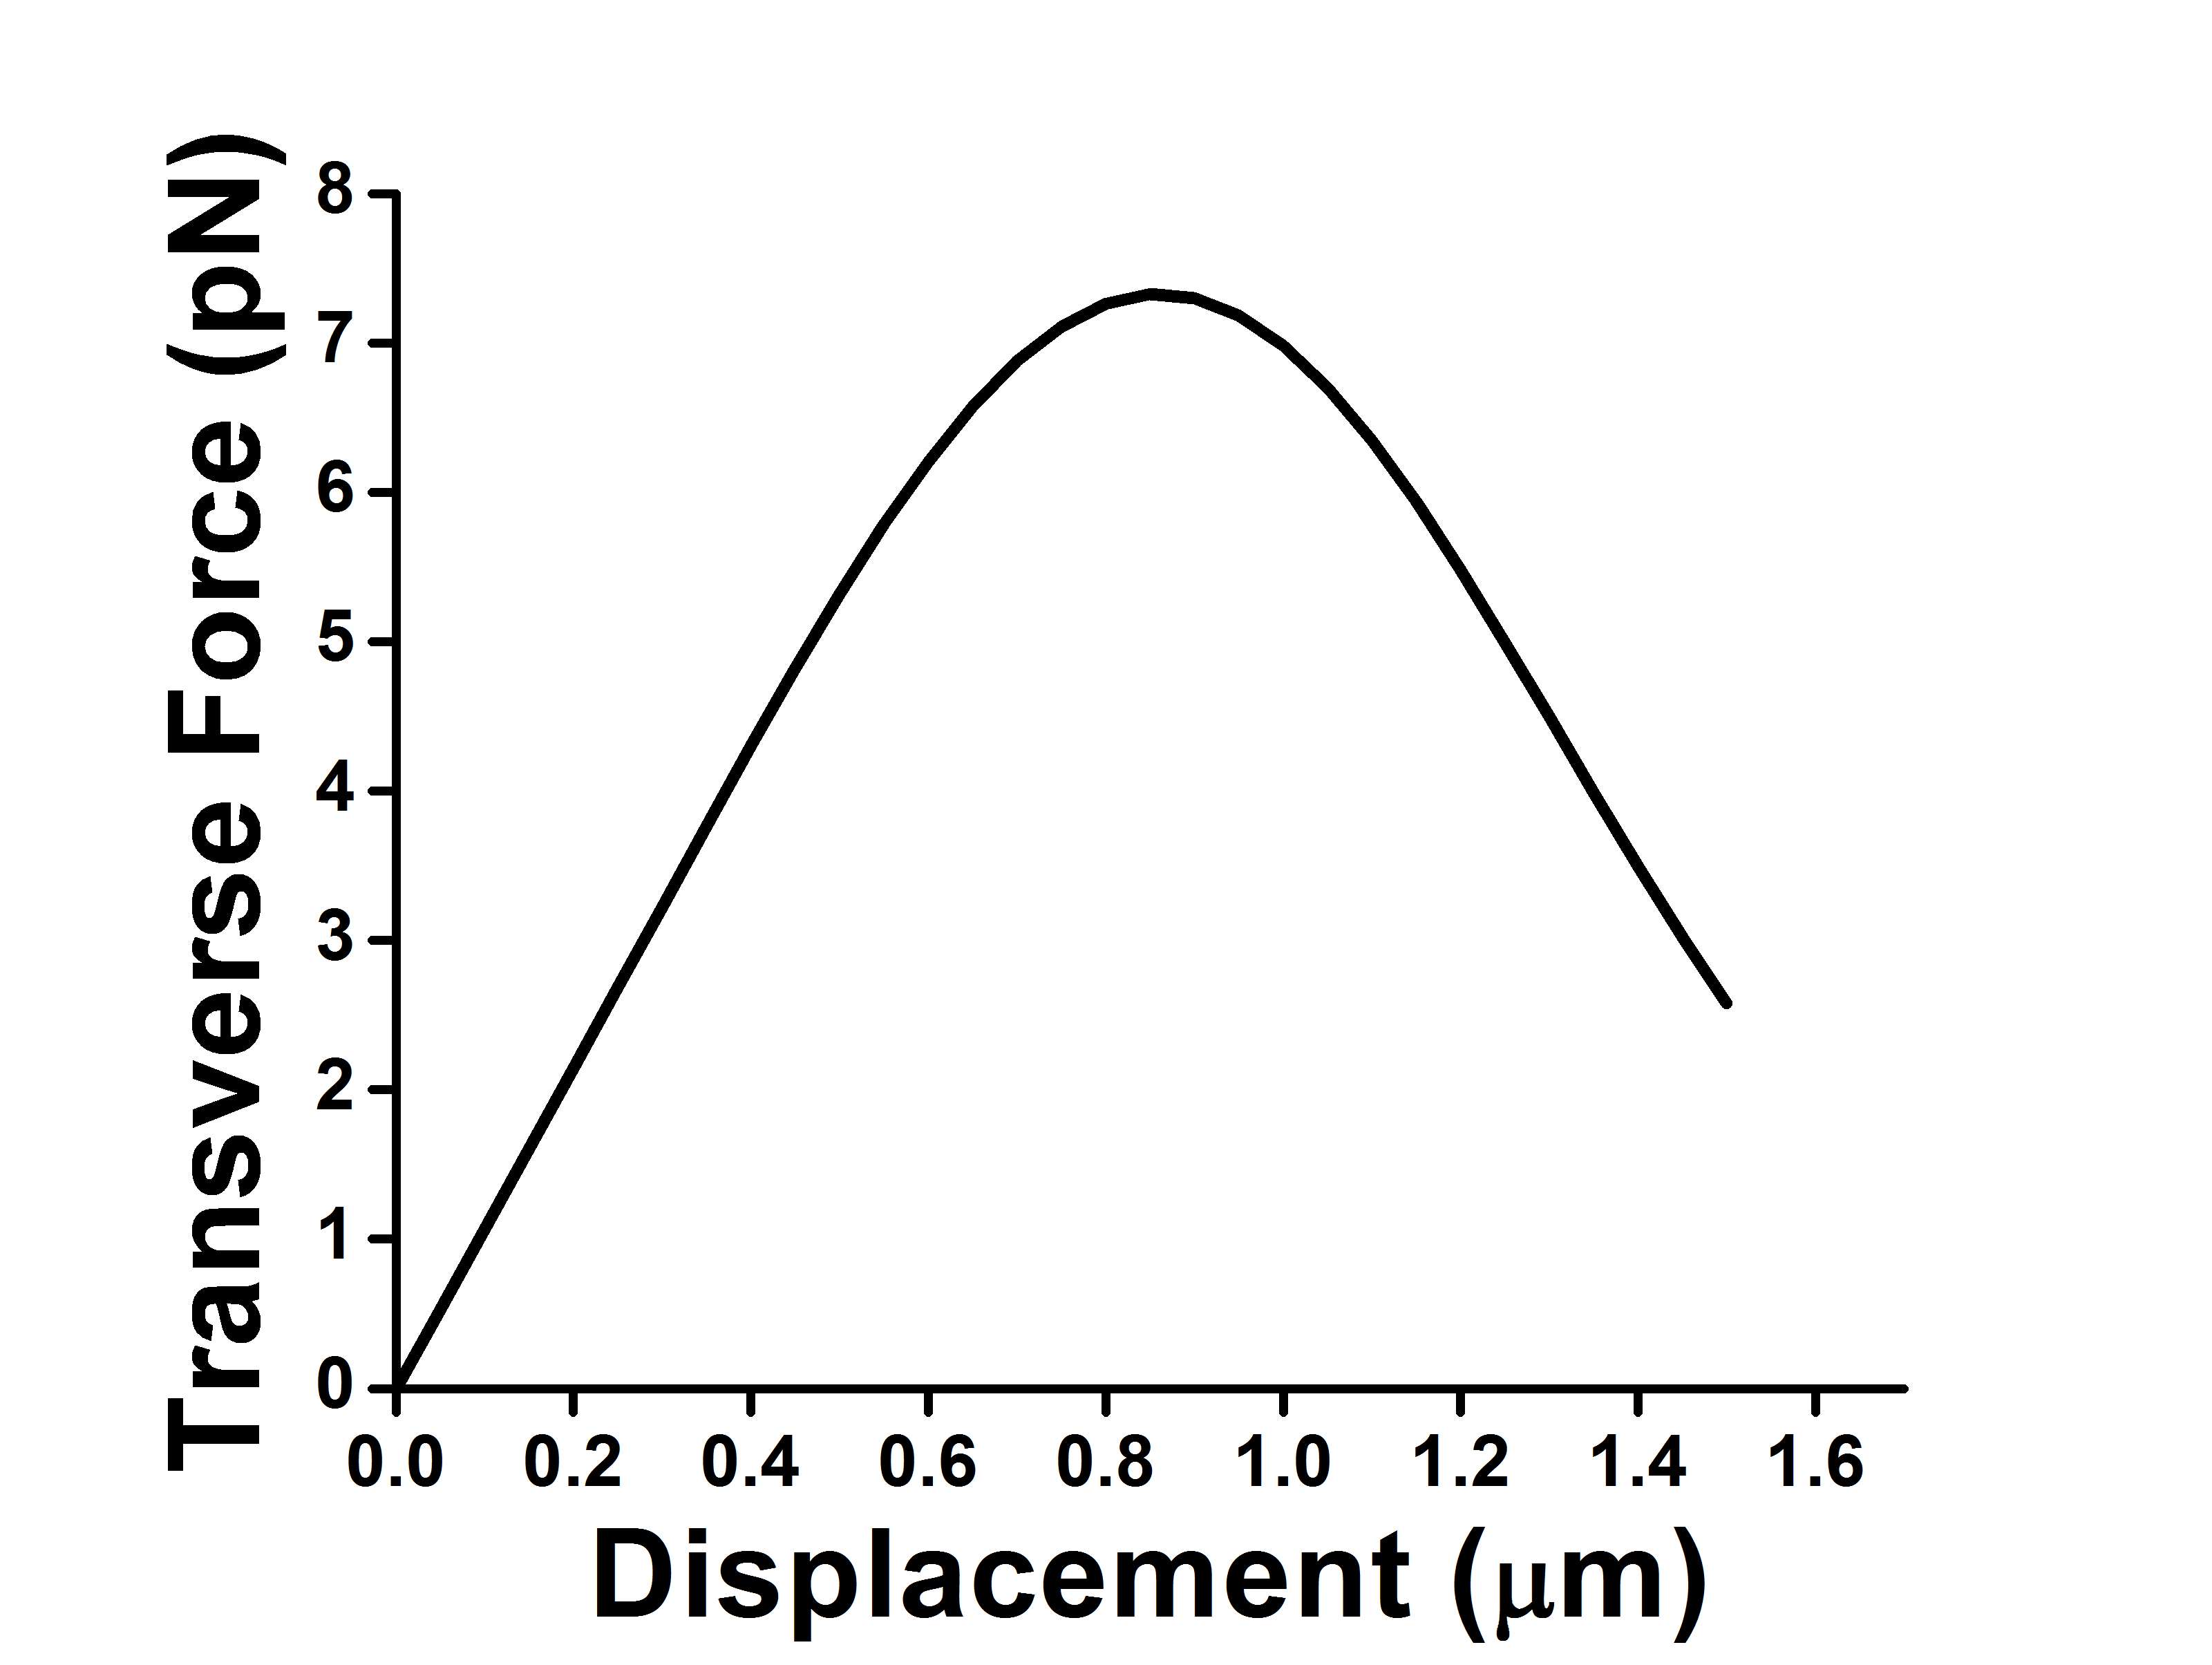
\includegraphics[width=4in]{appendix2/FvsL}
\caption[Restoring force on Bead Handles]{Restoring force on a glass bead (index of refraction 1.55, \SI{1000}{\nano\meter} radius) exerted by the HOT for various displacements from trap center. Calculations were performed using previously published software\cite{Nahmias2002}.}
\label{fig:BHforce}
\end{figure}

\clearpage

\chapter{Solutions to the heuristic model for ToW probability}

\begin{figure}
\centering
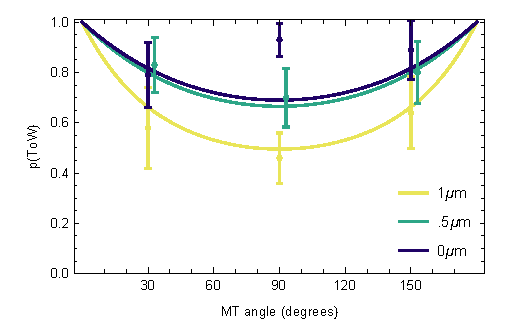
\includegraphics[width=12cm]{appendix2/heuristicEXP.pdf}
\caption[Solutions to the heuristic model for ToW probability]{Solutions to the heuristic model for ToW probability \\
A heuristic model (given in equation \ref{eq:rate_war}) poses the probability of undergoing ToW as the the probability of the cargo binding (with constant binding rate) to the crossing MT before leaving the ToW zone (see equation \ref{eq:ToW_zone} and figure \ref{fig:heuristic}). 
%Solutions to the model reproduce qualitative features of the simulated ToW probability for \SI{.5}{\micro\meter} and \SI{1}{\micro\meter} separation distances, shown in main text figure 4. The fact that the heuristic model does not qualitatively reproduce ToW probabilities for \SI{0}{\micro\meter} geometries highlights the importance of steric effects at these geometries. 
Solutions shown as solid curves. Bars represent 95\% confidence intervals for corresponding experimental data. Bars for data at \SI{.5}{\micro\meter} shifted slightly to aid the eye. Solutions plotted with $\kon^\text{macro}$ set to \SI{1}{\per\second}.
} \label{fig:heuristicEXP}
\end{figure}

\clearpage

\chapter{Empirical cumulative probability distributions for ToW times}

\begin{figure}
\centering
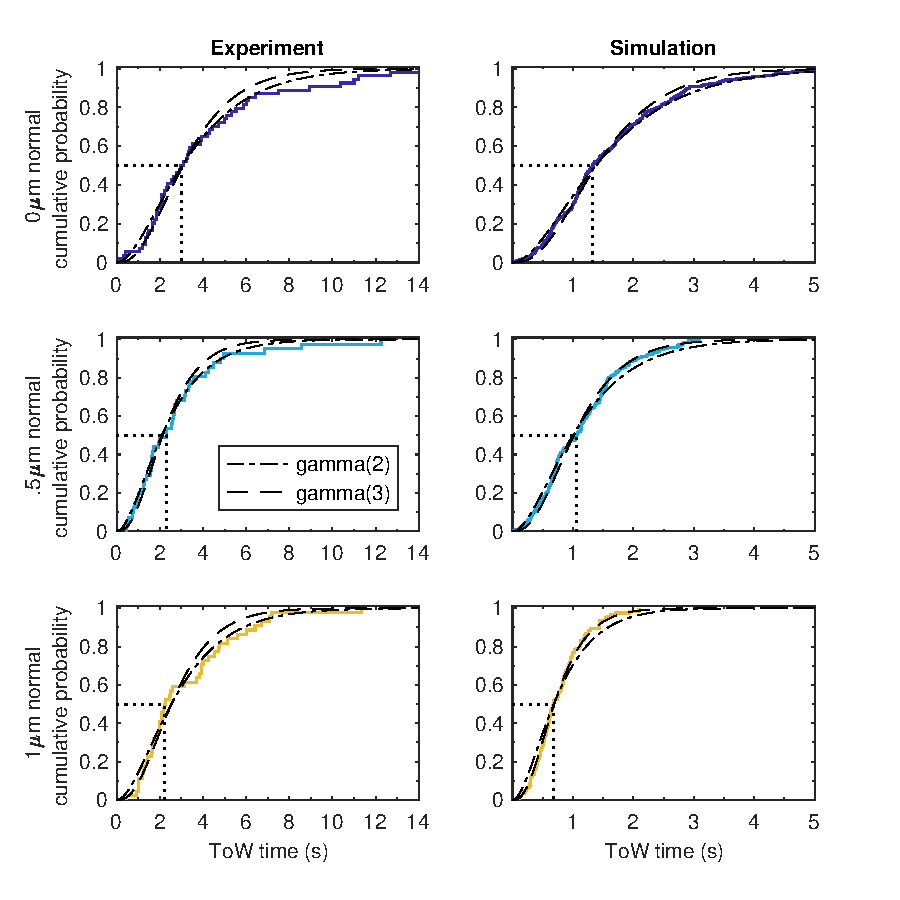
\includegraphics[width=6in]{appendix2/ToWtime_fits.pdf}
\caption[Empirical cumulative probability distributions for ToW times]{Empirical cumulative probability distributions for ToW times \\
The time for which cargos underwent ToW in 90 degree (normal) geometries was measured in experiments and simulations. Cumulative distributions are shown for each geometry. To aid interpretation, medians are highlighted with dotted lines. Fits to gamma cumulative distribution functions are shown in dashed lines. Good fits to gamma distributions with shape parameter 2-3 indicate distributions are well approximated as generated from 2-3 independent exponential events which we interpret as motor unbinding events.
} \label{fig:ToWtimes}
\end{figure}

\clearpage

\chapter{Number of motors engaged on MTs during ToW}

\begin{figure}
\centering
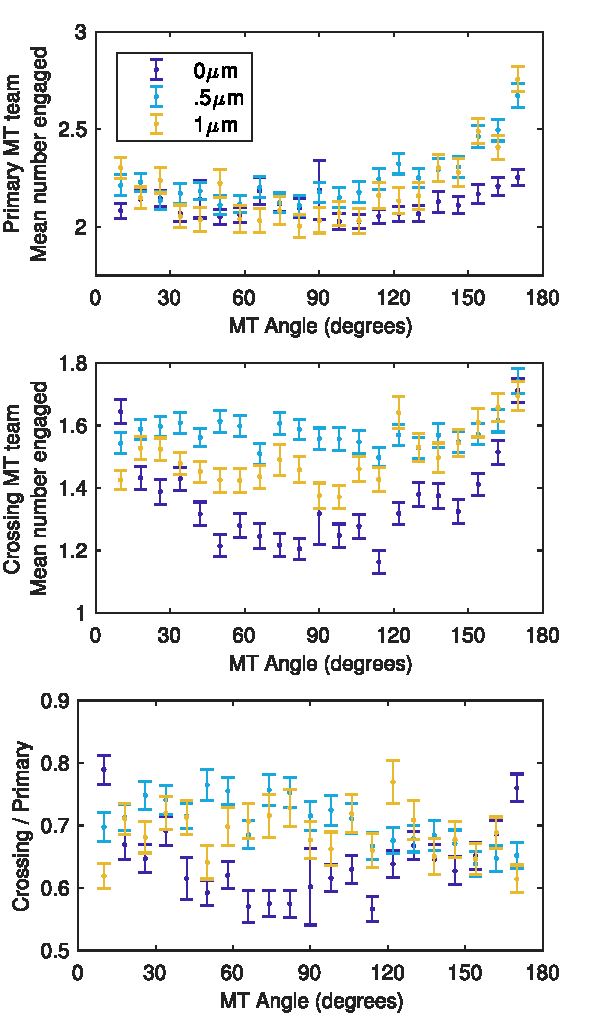
\includegraphics[width=4in]{appendix2/num_engagedEXP.pdf}
\caption[Number of motors engaged on MTs during ToW]{ Number of motors engaged on MTs during ToW\\
The mean number of motors engaged on the primary (\textit{top}) and crossing (\textit{center}) MTs during simulated ToWs are shown for each geometry. Additionally, the ratio of the mean number of motors engaged on the crossing MT to the mean number engaged on the primary MT is shown (\textit{bottom}). Data are represented as mean +/- SEM. Separation distances are colored as specified in the legend in the top panel.
} \label{fig:num_engagedEXP}
\end{figure}

\clearpage